Vamos a nombrar P a uno de los puntos de intersección de las circunferencias y vamos a trazar los siguientes radios:

\begin{center}
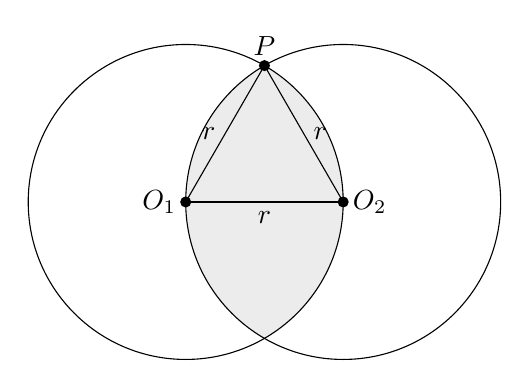
\begin{tikzpicture}
    % Definir el radio
    \def\r{2}

    % Sombrear el área de intersección
    \begin{scope}
        \clip (0,0) circle (\r);
        \fill[gray!15] (\r,0) circle (\r);
    \end{scope}

    % Dibujar la primera circunferencia
    \draw (0,0) circle (\r);

    % Dibujar la segunda circunferencia con un radio coincidente
    \draw (\r,0) circle (\r);

    % Marcar los centros de las circunferencias
    \fill (0,0) circle (2pt) node[left] {$O_1$};
    \fill (\r,0) circle (2pt) node[right] {$O_2$};
    
    \fill (\r/2, {\r*sqrt(3)/2}) circle (2pt) node[above] {$P$};

    % Dibujar el radio coincidente y etiquetarlo
    \draw (0,0) -- (\r,0) node[midway, below] {$r$};
    \draw (0,0) -- (\r/2, {\r*sqrt(3)/2}) node[midway, left] {$r$};
    \draw (\r,0) -- (\r/2, {\r*sqrt(3)/2}) node[midway, right] {$r$};
\end{tikzpicture}
\end{center}

Vemos que se forma el $\triangle O_1PO_2$ es equilátero de lado $r$, y su área es:

\[ A_{\triangle O_1PO_2} = \frac{\sqrt{3} \cdot r^2}{4} \]

La sección circular formada por ( $PO_1O_2$ ) es una porción del círculo con un ángulo de $60^\circ$, luego el área de esta sección circular es:

\[ A_{PO_1O_2} = \frac{\pi r^2}{6} \]

Dado que \( A_{PO_2O_1} = A_{PO_1O_2} \) y que el área sombreada es simétrica respecto a \( \overline{O_1 O_2} \), notemos que calcularse con la siguiente fórmula:

\[ A_{sombreada} = 4 \cdot A_{O_1PO_2} - 2 \cdot A_{\triangle O_1PO_2}\]

Simplificando y sustituyendo nos quedaría:

\[ A = \frac{2\pi r^2}{3} - \frac{\sqrt{3} \cdot r^2}{2} \]

Veamos el código en C\# para calcular esta fórmula:

\begin{lstlisting}
    Console.Write("Ingrese el radio r: ");
    double radius = double.Parse(Console.ReadLine());
    
    double intersectionArea = 2 * Math.PI * radius * radius / 3 
                                - Math.Sqrt(3) * radius * radius / 2;
    
    Console.WriteLine("El área sombreada es: " + intersectionArea);
\end{lstlisting}
